%\chapter{Recuperación de información: getStatus} \label{append:getStatus}

\begin{center}
    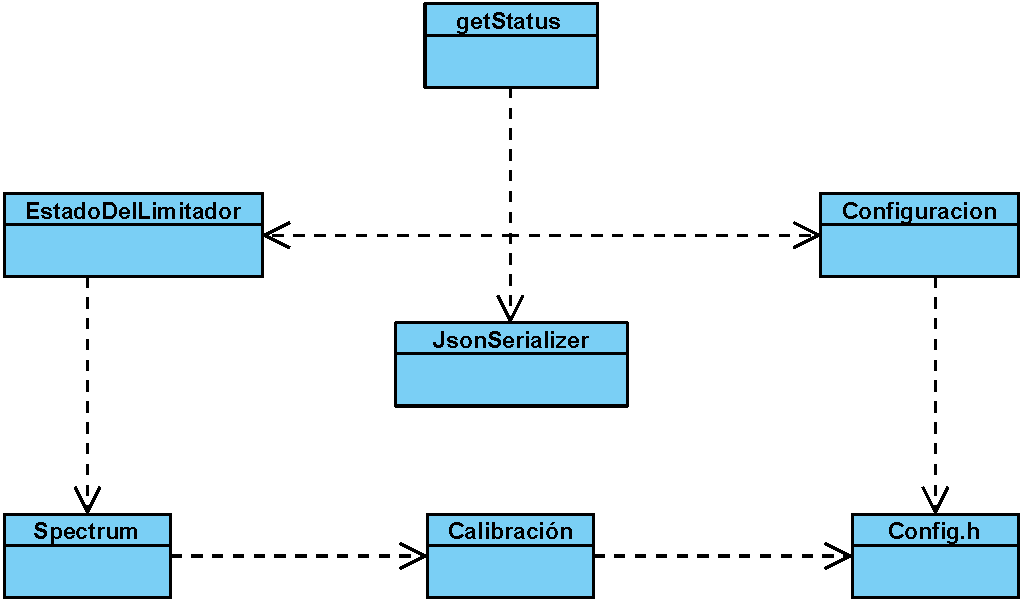
\includegraphics[width=0.9\textwidth]{figuras/lms11-getStatus.pdf}
    \captionof{figure}{Diagrama de clases del programa getStatus}
    \label{fig:getStatus}
\end{center}

El programa \verb|getStatus| devuelve información sobre el estado del limitador en el momento de la llamada. Para ello, lee el fichero \verb|/tmp/estado.slr| y devuelve su contenido en formato JSON. El fichero \verb|/tmp/estado.slr| es mantenido por el proceso de limitación en el caso del LM7, o por el proceso registrador en el caso del LM9 y el LM11.

En la figura \ref{fig:getStatus} se muestra el diagrama de clases simplificado del programa.

Los listados \ref{lst:lm7-getStatus} y \ref{lst:lm9-getStatus} muestran los esquemas JSON devueltos por este programa en cada una de las versiones. \\

\begin{lstlisting}[
    language=json,
    label={lst:lm7-getStatus},
    caption={Esquema JSON devuelto por getStatus en la versión LM7.}
]
{
  "definitions": {
    "data": {
      "type": "object",
      "properties": {
        "serialNumber": {
          "type": "string",
          "format": "integer"
        },
        "version": {
          "type": "string"
        },
        "time": {
          "type": "string"
        },
        "configTime": {
          "type": "string"
        },
        "place": {
          "type": "string"
        },
        "direction": {
          "type": "string"
        },
        "council": {
          "type": "string"
        },
        "responsible": {
          "type": "string"
        },
        "phoneNumber": {
          "type": "string"
        },
        "vendor": {
          "type": "string"
        },
        "deviceType": {
          "type": "string"
        },
        "leftline": {
          "type": "string"
        },
        "rightline": {
          "type": "string"
        },
        "microphone": {
          "type": "string"
        },
        "maximum": {
          "type": "string"
        },
        "microphoneConnected": {
          "type": "string"
        },
        "running": {
          "type": "string",
          "format": "integer"
        },
        "attenuation": {
          "type": "integer"
        },
        "micSpectrum": {
          "type": "array",
          "items": {
            "type": "number"
          }
        },
        "leftSpectrum": {
          "type": "array",
          "items": {
            "type": "number"
          }
        },
        "rightSpectrum": {
          "type": "array",
          "items": {
            "type": "number"
          }
        }
      }
    }
  }
}
\end{lstlisting}

\vspace{1em}

\begin{lstlisting}[
    language=json,
    label={lst:lm9-getStatus},
    caption={Esquema JSON devuelto por getStatus en las versiones LM9 y LM11.}
]
{
  "definitions": {
    "data": {
      "type": "object",
      "properties": {
        "time": {
          "type": "string",
          "format": "date-time"
        },
        "attenuation": {
          "type": "number"
        },
        "isActive": {
          "type": "boolean"
        },
        "running": {
          "type": "boolean"
        },
        "microphoneConnected": {
          "type": "boolean"
        },
        "maximum": {
          "type": "number"
        },
        "serialNumber": {
          "type": "string"
        },
        "version": {
          "type": "string"
        },
        "establishment": {
          "type": "string"
        },
        "address": {
          "type": "string"
        },
        "council": {
          "type": "string"
        },
        "responsible": {
          "type": "string"
        },
        "phonenumber": {
          "type": "string"
        },
        "configTime": {
          "type": "string"
        },
        "vendor": {
          "type": "string"
        },
        "deviceType": {
          "type": "string"
        },
        "noiseAttenuation": {
          "type": "number"
        },
        "noiseIsActive": {
          "type": "boolean"
        },
        "microphone": {
          "type": "number"
        },
        "leftline": {
          "type": "number"
        },
        "rightline": {
          "type": "number"
        },
        "mic": {
          "$ref": "#/definitions/spectrum"
        },
        "left": {
          "$ref": "#/definitions/spectrum"
        },
        "right": {
          "$ref": "#/definitions/spectrum"
        }
      }
    },
    "spectrum": {
      "type": "object",
      "properties": {
        "energy": {
          "type": "array",
          "items": {
            "type": "number"
          }
        },
        "dB": {
          "type": "array",
          "items": {
            "type": "number"
          }
        },
        "aWeighted": {
          "type": "array",
          "items": {
            "type": "number"
          }
        },
        "globaldB": {
          "type": "number"
        },
        "dBA": {
          "type": "number"
        }
      }
    }
  }
}
\end{lstlisting}

%Esquemas generados a partir de muestras JSON del programa, mediante el uso de las herramientas \url{www.json-schema.org} y \url{www.jsonschemavalidator.net}.